\chapter{导体与绝缘体}\label{ch:g4:conductors-insulators}

为什么电线用金属制成 --- 外面却包着塑料？
为什么开关里的小触片能导通电流，而它的
外壳却能保护你的手指安全？去年我们接通了回路；今年
我们要探究：电究竟能穿过哪些材料。
答案是把所有材料分为两类：导体和
绝缘体。

\section{检测器}

\begin{method}[搭建检测器]\label{met:g4:conductors-insulators:tester}
搭建去年的回路 --- 电池、导线、灯泡 --- 但要故意留出
一处缺口：两根导线的自由端相距一指宽。
\begin{enumerate}
  \item 将两个自由端接触：灯泡亮 ---
        检测器可以正常工作；
  \item 用待测物体跨接缺口，将其
        两个金属端分别紧压在两根导线上；
  \item 观察灯泡：亮表示电流穿过了物体；
        暗则表示电流无法通过。
\end{enumerate}
灯泡给出答案：当被测物体
接通回路时，灯泡恰好亮起。
\end{method}

\begin{omfigure}
\begin{tikzpicture}[scale=0.9]
  \draw (0,0) to[battery1, l=battery] (0,2.6)
    to[short] (2.2,2.6)
    to[lamp, l=bulb] (4.4,2.6)
    to[short] (6.0,2.6) -- (6.0,1.7);
  \draw (6.0,0.9) -- (6.0,0) to[short] (0,0);
  \fill (6.0,1.7) circle (1.6pt) node[right, font=\small]
    {~自由端};
  \fill (6.0,0.9) circle (1.6pt) node[right, font=\small]
    {~自由端};
  \draw[thick, fill=omMeth, fill opacity=0.4]
    (5.75,0.95) rectangle (6.25,1.65);
  \node[right, font=\small] at (6.6,1.3) {待测物体};
\end{tikzpicture}

{\small 检测器：一个带一处缺口的完好回路。任何搭接在缺口上的东西
都是正在被测试的对象 --- 灯泡显示电流
能否穿过它。}
\end{omfigure}

\section{导体与绝缘体}

\begin{definition}[导体]\label{def:g4:conductors-insulators:conductor}
称\emph{导体}\index{导体}为能让电流
通过的材料。在检测器中，跨接在缺口上的导体
会使回路闭合，灯泡亮起。
\end{definition}

\begin{definition}[绝缘体]\label{def:g4:conductors-insulators:insulator}
称\emph{绝缘体}\index{绝缘体}为能阻挡
电流通过的材料。用绝缘体跨接缺口，回路仍然
断开如故：灯泡保持不亮。
\end{definition}

\begin{example}[一上午的测试]\label{ex:g4:conductors-insulators:trials}
课堂检测结果：钢回形针 --- 亮。
硬币 --- 亮。厨房铝箔 --- 亮。钥匙 --- 亮。
塑料尺 --- 暗。木铅笔 --- 暗。玻璃弹珠
--- 暗。橡皮 --- 暗。纸条 --- 暗。
规律一目了然：能使灯泡亮的物体
全都由金属制成。
\end{example}

\begin{proposition}[金属导电]\label{prop:g4:conductors-insulators:metals}
所有金属都能导电 --- 铁、铜、铝、金，
每一种都能导电。磁铁对铁的挑剔让我们感到意外，
而检测器永远不会。日常生活中其他大多数固体 ---
如塑料、木头、玻璃、橡胶、纸和蜡 --- 都是绝缘体。
\end{proposition}

\begin{remark}[导体并不都有磁性]\label{rem:g4:conductors-insulators:notmagnet}
不要混淆两种金属特性。磁铁只选择铁
及其同族金属；电流则宽容得多，
流经\emph{每一种}金属。被磁铁忽略的铝箔
仍能很好地导电 --- 两种不同的游戏，
两套不同的规则。
\end{remark}

\section{导体与绝缘体协同工作}

\begin{example}[导线的构造]\label{ex:g4:conductors-insulators:wire}
看看台灯电线与插头相连的一端：内部
是闪亮的铜芯 --- 导体，即电流的通道；外面
包着彩色塑料 --- 绝缘体，即通道的围栏。铜芯
承担导电的任务；塑料把电流留在里面，你的
手指则被挡在外面。家中每根电缆都将两者搭配：导体
包在绝缘体之中。
\end{example}

\begin{omfigure}
\begin{tikzpicture}[scale=0.85]
  \draw[thick, fill=omExo, fill opacity=0.25]
    (0.5,0.35) rectangle (6.5,1.65);
  \draw[thick, fill=omThm, fill opacity=0.45]
    (0.5,0.78) rectangle (7.6,1.22);
  \node[right, font=\small] at (8.35,1.8) {塑料护套：绝缘体};
  \draw[-Stealth, omExo] (8.3,1.8) -- (6.3,1.55);
  \node[right, font=\small] at (8.35,1.0) {铜芯：导体};
  \draw[-Stealth, omExo] (8.3,1.0) -- (7.72,1.0);
\end{tikzpicture}

{\small 剥去外皮的电缆：铜制通道供电流通过，
外面是起保护作用的塑料围栏。}
\end{omfigure}

\begin{omfigure}
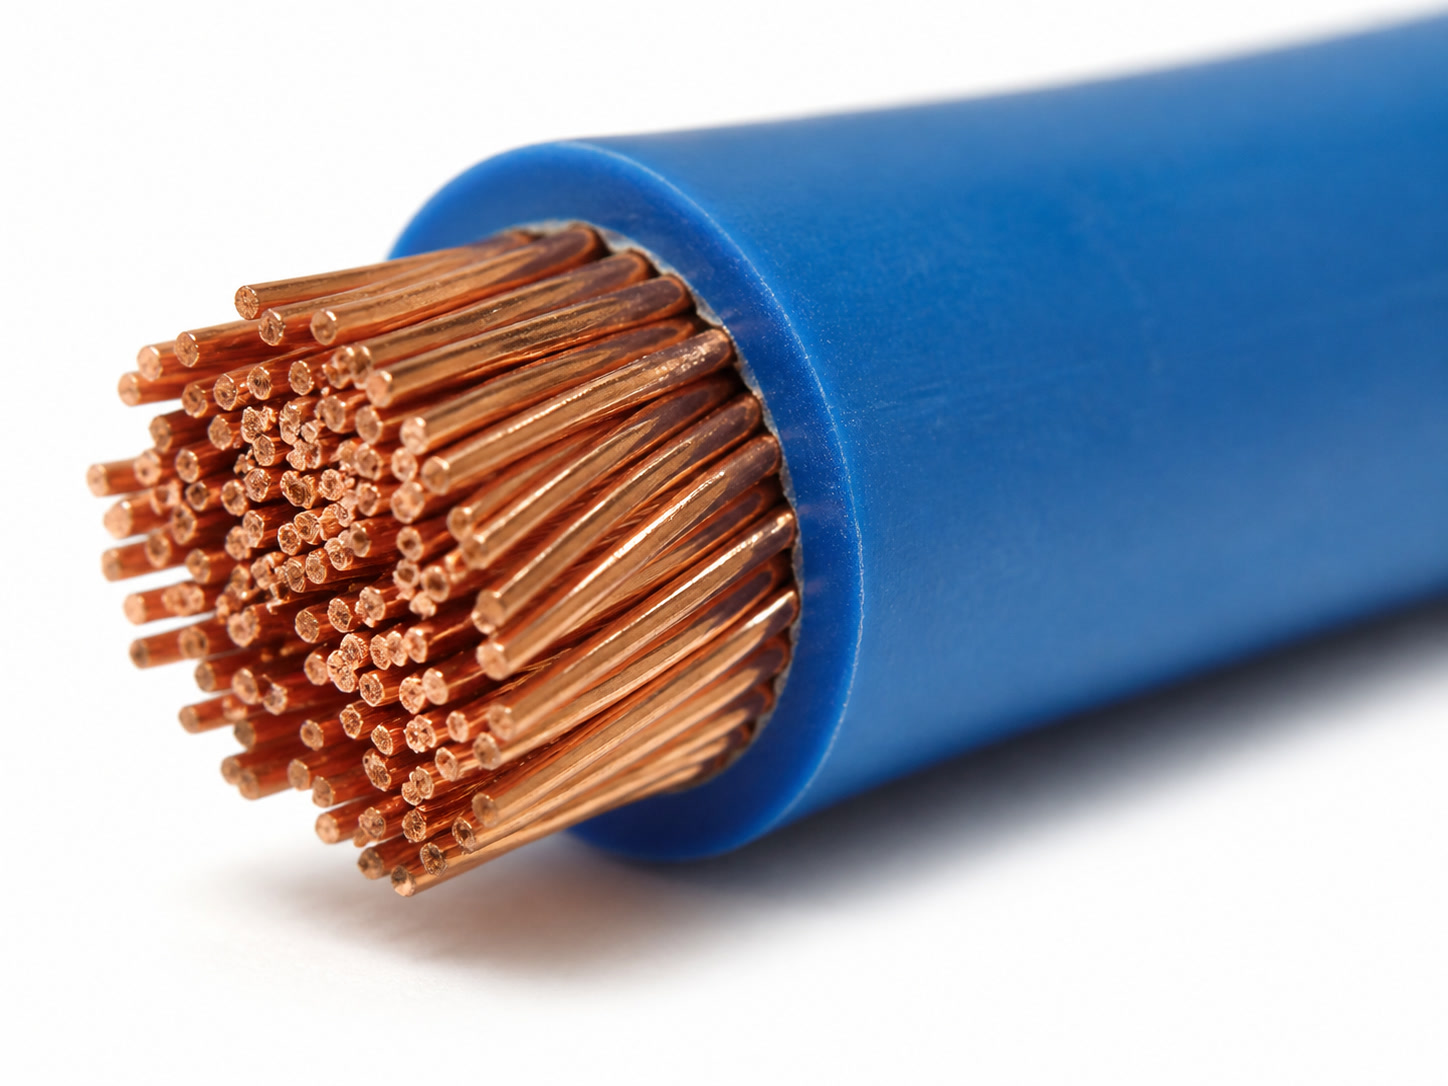
\includegraphics[width=0.5\linewidth]{images/book1/ai/g4-conductors-cable.jpg}

{\small 剪断的电缆端面，真实可见：闪亮的铜丝 --- 导体 --- 包在彩色塑料护套里 --- 绝缘体。}
\end{omfigure}

\begin{example}[认识日常物品]\label{ex:g4:conductors-insulators:objects}
许多设计本身就能说明道理。开关：金属桥（它
必须导电）装在塑料外壳里（你的手指不能导电）。
电工用的螺丝刀：钢制刀头，粗厚的绝缘手柄。
插座：深处是金属，外面是塑料面板。高压输电塔把裸露的金属电缆
架在很高的地方，电缆挂在长长的绝缘圆盘上，
以防电流漏入塔身。
\end{example}

\begin{remark}[水、人与安全规则的由来]\label{rem:g4:conductors-insulators:safety}
还有一种导体需要说明：\emph{潮湿的
物体} --- 包括潮湿的人体皮肤。人体导电很差，但
墙上插座的电压如此之大，“差”也已绰绰有余。这正是你所熟知的安全规则背后的深层原因：
不要把东西捅进插座，不要用湿手触摸任何带电的东西，
不要让吹风机靠近浴缸。电池测试器
之所以安全，\emph{因为}
电池的推动力很小；插座则毫不留情。
\end{remark}

\section{练习}

\begin{exercise}[$\star$]\label{exo:g4:conductors-insulators:1}
什么是导体？什么是绝缘体？哪一种能使测试器的
灯泡亮起？
\end{exercise}

\begin{exercise}[$\star$]\label{exo:g4:conductors-insulators:2}
将下列物品分为导体和绝缘体：钢勺；\ 软木塞；\ 厨房锡箔纸；\
玻璃杯；\ 铜币；\ 塑料块。
\end{exercise}

\begin{exercise}[$\star$]\label{exo:g4:conductors-insulators:3}
在任何测试之前，你如何检查测试器本身是否正常？
为什么这一检查很重要？
\end{exercise}

\begin{exercise}[$\star$]\label{exo:g4:conductors-insulators:4}
某个待测物体使灯泡不亮。请给出两种可能的原因——
一种与物体本身有关，一种与马虎的测试有关。
\end{exercise}

\begin{exercise}[$\star$]\label{exo:g4:conductors-insulators:5}
为什么台灯电线内部用铜、外层用塑料？
每种材料各起什么作用？
\end{exercise}

\begin{exercise}[$\star$]\label{exo:g4:conductors-insulators:6}
开关中，哪一部分是导体，哪一部分是
绝缘体？为什么它两者都需要？
\end{exercise}

\begin{exercise}[$\star$]\label{exo:g4:conductors-insulators:7}
铝箔完全不被磁铁吸引。它能让测试器的
灯泡亮起吗？哪条规则可以作答，以及
\cref{rem:g4:conductors-insulators:notmagnet}提醒要避免哪种混淆？
\end{exercise}

\begin{exercise}[$\star$]\label{exo:g4:conductors-insulators:8}
铅笔由木头和石墨笔芯构成。尼诺的测试器
在涂漆的木头两端一直不亮，但从一端到另一端穿过削尖的石墨时会微微发亮。
尼诺发现了铅笔两种材料的什么
特性？
\end{exercise}

\begin{exercise}[$\star$]\label{exo:g4:conductors-insulators:9}
为什么电工用的螺丝刀和钳子要有粗厚的塑料
手柄？哪种材料在保护谁？
\end{exercise}

\begin{exercise}[$\star\star$]\label{exo:g4:conductors-insulators:10}
一条项链链条使测试器显示“亮”；一条木珠项链显示“暗”；
一条金属珠子打结串在粗棉绳上的项链也显示“暗”——
尽管每颗珠子都能导电！
请沿着电流的路径，
从一颗珠子到下一颗，解释第三种结果。
\end{exercise}

\begin{exercise}[$\star\star$]\label{exo:g4:conductors-insulators:11}
为什么用湿手接触带电物体比用干手危险得多？
另外，为什么电池测试器可以安全地用于你的实验，
而插座永远不安全？请利用
\cref{rem:g4:conductors-insulators:safety}。
\end{exercise}
